%%%%%%%%%%%%%%%%%%%%%%%%%%%%%%%%%%%%%%%%%
% a0poster Portrait Poster for LiRI/UZH
% LaTeX Template
% Version 1.0 (22/06/13)
% Version 2.0 (08/04/22)
%
% The a0poster class was created by:
% Gerlinde Kettl and Matthias Weiser (tex@kettl.de)
% adapted by Danny McDonald for LiRI/UZH (mcddjx@gmail.com)
%
% License:
% CC BY-NC-SA 3.0 (http://creativecommons.org/licenses/by-nc-sa/3.0/)
%
%%%%%%%%%%%%%%%%%%%%%%%%%%%%%%%%%%%%%%%%%

\documentclass[a0,portrait]{a0poster}

\usepackage{hyperref}
\usepackage{colortbl}

% control margins here
\usepackage{geometry}
 \geometry{
 a0paper,
 left=5cm,
 top=4.5cm,
 right=5cm,
 bottom=4.5cm
 }
\addtolength{\textwidth}{4.5cm} % width of text can be adjusted if margins above are adjusted

\usepackage{multicol} % This is so we can have multiple columns of text side-by-side
\columnsep=3em % This is the amount of white space between the columns in the poster
\columnseprule=0pt % This is the thickness of the black line between the columns in the poster

% UZH colours
\usepackage[svgnames]{xcolor}
\definecolor{uzhblau100}{RGB}{0, 40, 165}
\definecolor{uzhblau80}{RGB}{51,83,183}
\definecolor{uzhockerrot100}{RGB}{220, 96, 39}
\definecolor{uzhockerrot80}{RGB}{227, 128, 82}
\definecolor{uzhflaschengruen100}{RGB}{42, 127, 98}
\definecolor{uzhflaschengruen80}{RGB}{86, 157, 133}
\definecolor{conclusion}{RGB}{204,212,237} % the conclusion box colour

\usepackage{ifthen} % needed to stop horizontal line above 'Conclusions' section
\usepackage{graphicx} % Required for including images
\graphicspath{{figures/}} % Location of the graphics files
\usepackage{mwe,tikz}\usepackage[percent]{overpic} % overlay your photo over the background
\usepackage{booktabs} % Top and bottom rules for table
\usepackage[font=small,labelfont=bf]{caption} % Required for specifying captions to tables and figures
\usepackage{amsfonts, amsmath, amsthm, amssymb} % For math fonts, symbols and environments
\usepackage{wrapfig} % Allows wrapping text around tables and figures

\usepackage{fontspec} % custom fonts
\defaultfontfeatures[Palatino]
{
    Extension = .ttf,
    UprightFont = font/LT_41167,
    BoldFont = font/LT_41169,
    ItalicFont  = font/LT_41168,
    BoldItalicFont = font/LT_41170,
}
\defaultfontfeatures[TheSans]
{
    Extension = .otf,
    UprightFont = font/TheSans-LP5Plain,
    BoldFont = font/TheSans-LP7Bld,
    ItalicFont  = font/TheSans-LP5PlainIT,
    BoldItalicFont = font/TheSans-LP7BldIT,
}
\setmainfont{TheSans} % choose your font here
\usepackage[onehalfspacing]{setspace} % remove for single spacing
\usepackage{tcolorbox} % for the conclusions box
\usepackage{blindtext} % you can remove this once you add your content
\usepackage[export]{adjustbox} % allow floating a graphic right
\usepackage{titlesec} % customising section titles
\usepackage{needspace} % prevent break between line and section title
\usepackage{nameref} % package and command to get the name of the current section (for ifthen)

\begin{document}

% define how our section titles will look (with ruled line)
\titleformat{\section}
  {\needspace{1\baselineskip}\sectionrule\huge\bfseries}
  {\color{uzhblau100}\thesection.}
  {1em}
  {\color{uzhblau100}}

% draw horizontal line before section unless it is conclusions (if you change name of Conclusions, you should
% also change it here too so it is recognised and the line suppressed
\makeatletter
\newcommand{\sectionrule}{%
 \ifthenelse{\equal{\@currentlabelname}{Conclusions}}
 % use the below line instead of the above if conclusions is a section*
 % \ifthenelse{\equal{\@currentlabelname}{}}
  {}
  {\vspace*{-\baselineskip}
   \vrule height 1pt depth 1pt width \linewidth\vskip0.4pt
   \bigskip}%
}
\makeatother


%----------------------------------------------------------------------------------------
%	POSTER HEADER 
%----------------------------------------------------------------------------------------
%\title{Creating a \LaTeX{} poster template matching UZH specifications for LiRI presentations}
\title{Achieving the net-zero target:\\A meta-analysis of Turkish energy and climate scenarios}

% the top logo (in english!) and unit title
\noindent
\begin{minipage}{.15\linewidth}
 
\includegraphics[height=10cm]{hu.pdf}
\end{minipage}%
\begin{minipage}{.15\linewidth}
 
\includegraphics[height=10cm]{au.pdf}
\end{minipage}%
\begin{minipage}{.15\linewidth}
 
\includegraphics[height=10cm]{dtu.pdf}
\end{minipage}
\vspace{4em}

% The header is divided into two boxes, on the left is the text and on the right is the image
\begin{minipage}[b][][t]{.6\linewidth}
\vfill
\makeatletter
\raggedright{\fontsize{92pt}{100pt}\selectfont\color{uzhblau100}\textbf{{\@title}}\par}
\makeatother
\color{Black}
\vspace{1cm}
%\Huge\textit{Subtitle goes here}\\[2.4cm] % Subtitle if it exists
\underline{Gorkem Gungor\textsuperscript{1}}, {Latife Demirtas\textsuperscript{2}}, {Ramazan Sari\textsuperscript{3}}\\
\vspace{0.2cm}
\textsuperscript{1}Hacettepe University, Turkey.
\texttt{ggungor@enerji.gov.tr}\\
\textsuperscript{2}Ankara University, Turkey.\\
\textsuperscript{3}Technical University of Denmark, Denmark.
%\\ % add your institution
%\texttt{you@uzh.ch}%\\ % add your email
\end{minipage}%
%
\begin{minipage}[b][][t]{0.39\linewidth}
\vfill
  \begin{overpic}[width=.8\textwidth,right]{LIRI_WissPoster_Wasserzeichen.png} % what even is this thing?
     \put(85,0){\includegraphics[scale=2]{Gungor_photo.jpg}}  % your image goes in here
  \end{overpic}
\end{minipage}
\vspace{1cm}

%----------------------------------------------------------------------------------------
%	POSTER BODY
%----------------------------------------------------------------------------------------

\begin{multicols}{3} % This is how many columns your poster will be broken into

%----------------------------------------------------------------------------------------
%	INTRODUCTION
%----------------------------------------------------------------------------------------

\section{Introduction}

\Large 

The Ministry of Energy and Natural Resources Turkish National Energy Plan modeling horizon is 2035 and based on the net-zero target in 2053. The energy and climate scenarios included in the official reports are: 

\begin{itemize}
\item Energy Security Scenario (MENR, 2022)
\item Baseline and Net-Zero Scenarios (IPC, 2022), and 
\item Baseline, Optimistic and Pessimistic Scenarios (Akalın et al., 2012). 
\end{itemize}

The capacity projections in the Energy Security Scenario (MENR, 2022) are illustrated in Table 1 with data from Baseline and Net-Zero Scenarios (IPC, 2022) given in parantheses.

\begin{center}
 \vspace{2cm}
 \begin{tabular}{c c c c c} 
  \toprule
  Installed & unit & 2030 & 2035 & 2055 \\ [0.5ex] 
  capacity &&&& \\
  \midrule
  \rowcolor{LightCyan}
  Solar power & GW &  & 52.9 (59.7) & \\ 
  Wind power & GW &  & 29.6 (50.1) & \\
  \rowcolor{LightCyan}
  Nuclear power & GW &  & 7.2 (4.8) & \\
  New installed & GW &  & 96.9 & \\
  capacity &&&& \\
  \rowcolor{LightCyan}
  Total installed & GW &  & 189.7 (202.1) & \\
  \rowcolor{LightCyan}
  capacity &&&& \\
  Battery storage & GW &  & 7.5 & \\
  \rowcolor{LightCyan}
  Electrolyser & GW & 1.9 & 5.0 & 70.0 \\
  Demand side & GW & 0.9 & 1.7 & \\
  management &&&& \\
  \bottomrule
 \end{tabular}
\captionof{table}{Capacity projections from Energy Security Scenario (MENR, 2022) and Baseline and Net-Zero Scenarios (IPC, 2022) (in parantheses)}
\vspace{2cm}
\end{center}

%----------------------------------------------------------------------------------------
%	SECTIONS
%----------------------------------------------------------------------------------------

\section{Carbon emissions}

The Energy Security Scenario (MENR, 2022), illustrated in Figure 1, shows a peak fossil year of 2030 and a rapid expansion of renewable energy and nuclear power beyond 2050. 

\begin{center}\vspace{1cm}
    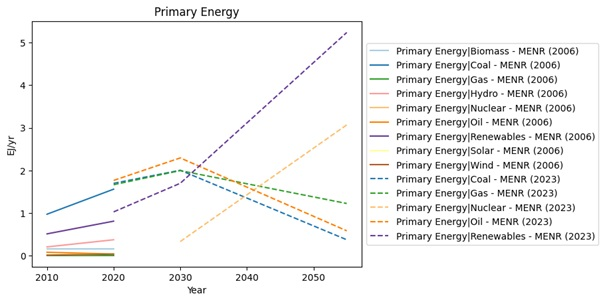
\includegraphics[width=1.0\linewidth]{Figure_1}
    \captionof{figure}{Primary energy supply projections from Turkish national plans}
\end{center}\vspace{1cm}

Estimated CO2 emissions from the official reports are illustrated in Figure 2. MENR (2023) is related with the NDC of Turkey (MoEUCC, 2023). Gungor and Sari (2020) assess the role of nuclear power for climate change mitigation strategy of Turkey. IPC (2022) net-zero scenario combines multiple energy supply and demand policies with labor market policies for a just low-carbon transition. Supply or market based strategies shift the emissions towards saturation, whereas multiple scenarios are required to achive the net-zero target. 

\begin{center}\vspace{1cm}
    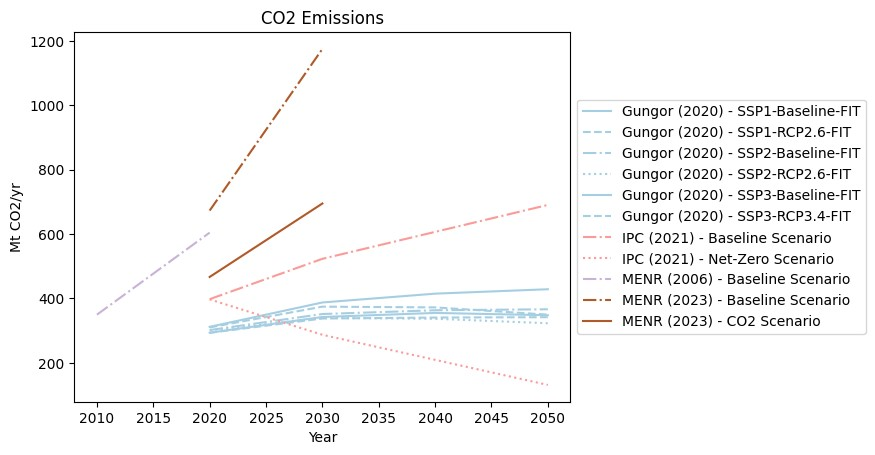
\includegraphics[width=1.0\linewidth]{Figure_2}
    \captionof{figure}{Carbon emission pathways}
\end{center}\vspace{1cm}

%----------------------------------------------------------------------------------------
%	CONCLUSIONS BOX
%----------------------------------------------------------------------------------------

%\section*{} % this dummy section draws a horizontal line above conclusions

\begin{tcolorbox}[width=1.0\linewidth,colback={conclusion},frame empty]
\section{Data availability}

The data and scripts are available at \href{https://github.com/gorkemgungormetu/turkish\_energy\_and\_climate\_pathways.git}{GitHub repository} under the Apache-2.0 License.

\end{tcolorbox}    

%----------------------------------------------------------------------------------------
%	FORTHCOMING RESEARCH
%----------------------------------------------------------------------------------------

\section{Categorization of scenarios by their fossil fuel shares}

Although the fossil fuel reserves are modest in Turkey, their share in primary energy supply is above 80\% (OECD, 2020). The expansion of renewable energy requires the electrification of hard-to-abate sectors such as industry, residential and transport. The authors select the share of coal as meta-data. The primary energy supply illustrated in Figure 3 shows trade-off between reduction in CO2 emissions and savings in primary energy supply in all scenarios.

\begin{center}\vspace{1cm}
    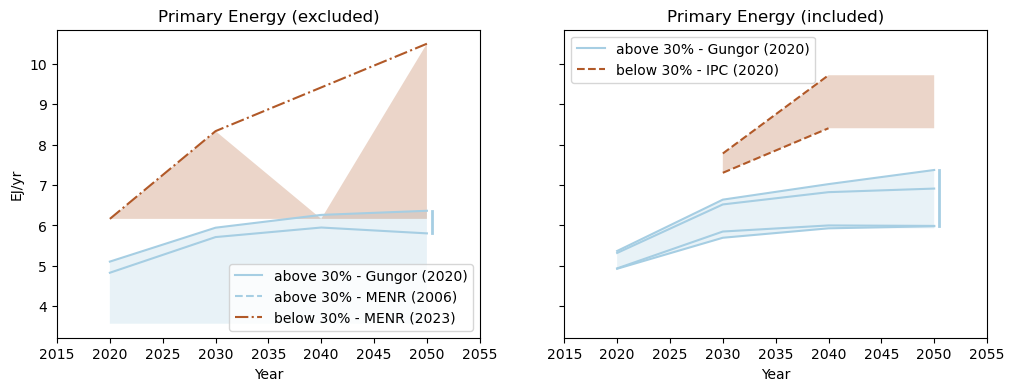
\includegraphics[width=1.0\linewidth]{Figure_3}
    \captionof{figure}{Primary energy supply, including (left) and excluding (right) extremely high and low emission scenarios}
\end{center}\vspace{1cm}


%----------------------------------------------------------------------------------------
%	REFERENCES
%----------------------------------------------------------------------------------------
\singlespacing
\small
\nocite{*} % Print all references regardless of whether they were cited in the poster or not
\bibliographystyle{plain} % Plain referencing style
\bibliography{sample} % Use the example bibliography file sample.bib

%----------------------------------------------------------------------------------------

\end{multicols}
\end{document}